%\addcontentsline{toc}{chapter}{Kapitel-1}
\chapter{Grundlage \label{kap0}}



\section{Definition \label{kap0_def}}
In der Absicht, bestimmte Probleme zu vermeiden, die sich aus der semantischen Verwirrung bestimmter Wörter oder Ausdrücke ergeben und die später während des Lesens dieser Arbeit auftreten könnten. Wir machen uns hier die Mühe, diese Wörter oder Ausdrücke, die immer wieder verwendet werden, in diesem Kontext zu definieren.

\begin{itemize}
	\item \textbf{Partikel/Teilchen}\\
	Laut Pons Wörterbuch, ein Partikel ist ``ein sehr kleines Teilchen von etwas''. Nun im Rahmen unserer Arbeit ist eine Partikel, jedes bewegliche oder unbewegliche Objekt oder Element, das auf einem Bild zu sehen ist.
	
	\item \textbf{Erkennung/Lokalisierung}\\
	Unter Erkennung wird hier gemeint, der Prozess, der es ermöglichen soll, jegliche auf ein Bild existierende Partikel zu detektieren/finden und ggf. zu umzingeln. Bei der Erkennung liegt der Fokus auf das Finden von Partikeln auf einem einzigen Bild.
	 
	\item \textbf{Verfolgung/Tracking}\\
	Bei der Verfolgung handelt es sich um einen Prozess, bei dem die vorhandenen Partikel gefunden werden. Dies geschieht jedoch nicht auf einem einzelnen Bild wie bei der Erkennung, sondern auf einer Sequenz von Bildern. So kann man den Verlauf (Historie) eines Partikels von Bild $1$ bis Bild $n$ erhalten. $n$ ist das letzte Bild der Bildsequenz.

	
	\item \textbf{Trajektorie/Verbindung/Verlinkung lokalisierter Partikel}\\
	Hierbei handelt es sich um die Verbindungslinie zwischen den Punkten, die die Position der Partikel im Laufe der Zeit (der Bilder) in der Bildsequenz darstellen. So kann man für ein Partikel in jedem Bild unterschiedliche Koordinaten (x,y) haben, vorausgesetzt, das Partikel ist beweglich.
	
%	\item \textbf{Bild/Image}\\
%	Ein Bild, genauer gesagt ein digitales Bild, bezeichnet eine Matrix oder ein Array von quadratischen Pixeln, die in Zeilen und Spalten geordnet sind. 
	
%	\item \textbf{Pixel}\\
%	Ein Pixel wird als kleinste Einheit (quadratisch) eines digitalen Bildes oder einer Grafik bezeichnet, die auf einem digitalen Bildschirm angezeigt werden kann.	
	
%	\item \textbf{Video}\\
%	Ein Video \cite{diff_imag_vs_video} ist eine Sequenz/Abfolge von Bildern  (so genannte Frames), die in einer bestimmten Frequenz aufgenommen und eventuell angezeigt wird.	
	
	%\item \textbf{Auflösung}
	
\end{itemize}

\section{Bild- und Videoqualität \label{kap0_bildAndVideoQlt}}
Dieser Teil der Arbeit widmet sich der Klärung von Begriffen, die mit dem Bereich der Bildverarbeitung zusammenhängen (Auflösung, Pixel, Dichte, ...), so dass der Unterschied zwischen Bildern guter und schlechter Qualität gemacht werden kann.\\

Es ist wichtig, einige Begriffe zu verstehen, um über die Qualität von Bildern oder Videos sprechen zu können.

\begin{itemize}
	\item \textbf{Bild/Image}\\
	Ein Bild \cite{what_is_a_image}, genauer gesagt ein digitales Bild, bezeichnet eine Matrix oder ein Array von quadratischen Pixeln, die in Zeilen und Spalten geordnet sind. 
	
	\item \textbf{Pixel}\\
	Ein Pixel \cite{what_is_a_pixel} wird als kleinste Einheit (quadratisch) eines digitalen Bildes oder einer Grafik bezeichnet, die auf einem digitalen Bildschirm angezeigt werden kann.
	
	\item \textbf{Video}\\
	Ein Video \cite{diff_imag_vs_video} ist eine Sequenz/Abfolge von Bildern  (so genannte Frames), die in einer bestimmten Frequenz aufgenommen und eventuell angezeigt wird.
\end{itemize}

\subsection{Bild-/Imagequalität \label{kap0_imageQlt}}
Im Allgemeinen bezieht sich die Qualität eines Bildes/Videos auf seine Auflösung. Das bedeutet, dass wir uns hier mit der Auflösung befassen, und noch besser, was diese ausmacht.
Wie bereits erwähnt, ist ein digitales Bild eine Darstellung von Pixeln, die in Höhe und Breite (Spalten und Zeilen) angeordnet sind.
Die Anzahl der Pixel, aus denen ein Bild besteht, sowie die Bittiefe dieser Pixel und die Art und Weise, wie sie verteilt sind, machen also einen Großteil der Auflösung eines Bildes aus.
Wir können also nicht nur über die Anzahl und Bittiefe der Pixel sprechen, sondern auch über ihre Dichte im Bild.\\

\subparagraph{Anzahl der Pixel\\}
Die Anzahl der Pixel kann einfach durch Multiplikation der Anzahl der Pixel in der Höhe mit der Anzahl der Pixel in der Breite bestimmt werden. Beispiel: Ein Bild mit (Höhe * Breite) $300 * 400  = 1200000$\textit{Pixel} oder $0,12$\textit{Megapixel}.

\subparagraph{Bilddichte\\}
Die Bilddichte wird jedoch in Pixel pro Zoll \textit{dpi} bzw.\textit{ppi} (pixel per inch) ausgedrückt. Das heißt, die Anzahl der Pixel, die pro Zoll angezeigt werden. Die Auflösung hängt also auch davon ab.  Je niedriger der Wert von \textit{dpi} ist, desto größer ist das Bild. Daher wird bei einem Bild mit wenigen Pixeln die Qualität bzw. Auflösung verringert, wie im folgenden Beispiel gezeigt wird. 
\begin{figure}[H]
    \centering
    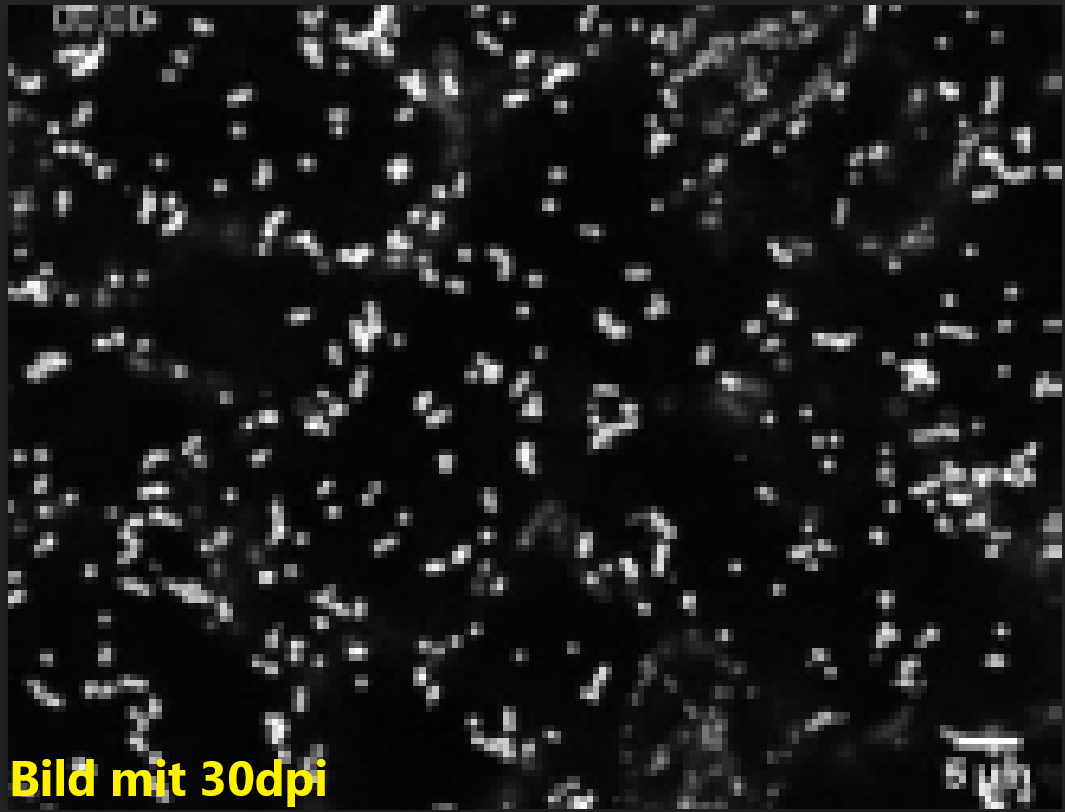
\includegraphics[width=1\textwidth]{Grafiken/trackpyBilder/30dpi.png}
    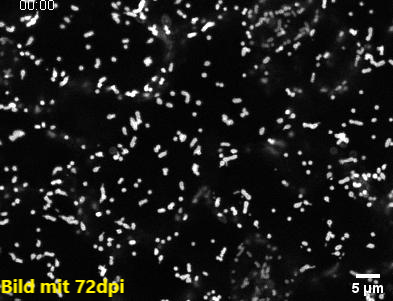
\includegraphics[width=1\textwidth]{Grafiken/trackpyBilder/72dpi.png}
    \caption{Vergleich zwischen Bild mit 72dpi und eins mit 30dpi.}
    \label{fig:kap0_72dpivs30dpi}
\end{figure}

\subparagraph{Bittiefe\\}
Die Bittiefe bezieht sich auf die Gesamtanzahl der Töne (Anzahl der Farben), die das Bild haben muss.  Die Gesamtzahl der Bittiefe wird durch gegeben:
\begin{equation}
	2^n = Bittiefe
\end{equation}   Dabei steht n für die Anzahl der Bits.
Je höher dieser Wert ist, desto mehr Farben werden gespeichert und angezeigt. Beispiel: Ein Bild mit einer Bittiefe von 1 Bit: $2^1=2$ kann nur zwei Farben speichern, nämlich Schwarz und Weiß.


\subsection{Videoqualität \label{kap0_videoQlt}}

Ein Video ist letztlich nur eine Folge von Bildern, die mit einer bestimmten Frequenz, nämlich Frames pro Sekunde (\textit{fps}), gerendert oder aufgenommen werden.
Je höher die Anzahl der \textit{fps}, desto flüssiger das Video.
Der Punkt über die Auflösung von Bildern \ref{kap0_imageQlt} sollte daher noch einmal gelesen werden, um das Konzept der Auflösung besser zu verstehen und auf ein Video anzuwenden.

\section{Verfahren  \label{kap0_verf}}
Zur Erkennung von Partikeln gibt es eine Vielzahl von Ansätzen. Zu diesen Ansätzen oder Methoden gehören: "Maxima detection", "thresholding", "fitting", "centroid estimation", wie in ''Objective comparison of particle tracking methods" erwähnt.
\subsection{Erkennung Methoden \label{kap0_verf_erkenn}}


\begin{itemize}
\item \textbf{Maxima detection}\\
Die "Maxima detection", auch "Peak detection'' oder "lokal maxima" genannt, ist ein Konzept, das es ermöglicht, innerhalb jeder Zeile eines Akkumulators oder Arrays in einem bestimmten Intervall das Element zu finden (im Allgemeinen ist die Position des Elements im Array die Mitte des gewählten Intervalls), das den höchsten Wert vor und nach ihm in diesem Intervall hat.  Die Werte in diesen Arrays sind in der Regel die Helligkeitsintensität jedes Punktes im Bild.\\
Beispiel: Das Array a = [74, 4, 5, 71, 70, 8, 9, 67] und ein Intervall von 5. Das zu findende Element ist auf Position 3 (Mitte des Arrays)


\begin{figure}[H]
    \centering
    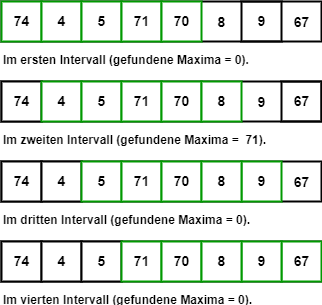
\includegraphics[width=1\textwidth]{Grafiken/grundlage/maxima Beispiel.png}
    \caption{Beispiel von `maxima detection'}
\end{figure}

Dies ermöglicht es, Schritt für Schritt die Bildpunkte mit der höchsten Helligkeit zu ermitteln, bei denen es sich wahrscheinlich um Partikel oder zu erkennende Elemente handelt.
"VK Yadav et al.'' beschreiben in ihrem Artikel Approach to accurate circle detection: ''Circular Hough Transform and Local Maxima concept'' (Ansatz zur genauen Kreiserkennung: ''Circular Hough Transform und lokales Maxima-Konzept'') 
\cite{yadav2014approach} eine explizitere Beschreibung.


\item \textbf{Thresholding}\\
Beim Thresholding wird jeder Pixelwert (Pixelintensität) in einem Bild mit einem bestimmten Schwellenwert (threshold) verglichen. Dadurch werden alle Pixel des Eingabebildes in zwei Gruppen unterteilt: Die Pixelgruppe mit Intensitätswerten unterhalb eines Schwellenwerts und eine mit Intensitätswerten über einem Schwellenwert.\\
Auf diese Weise ist es möglich, anhand der erhaltenen Pixelgruppen zu bestimmen, welche Bildelemente am ehesten mit den gesuchten Partikeln übereinstimmen und gegebenenfalls den Schwellenwert anzupassen.\\
Die Anwendungsmöglichkeiten werden in ''A Multi-Thresholding Algorithm for Sizing out of Focus Particles'' \cite{ju2012multi} und in ''A review of thresholding strategies applied to human chromosome segmentation'' \cite{poletti2012review} besprochen und implementiert.


\item \textbf{Fitting}\\
Das Fitting ist eine Funktion, die in der Regel im Bereich des maschinellen Lernens eingesetzt wird. Die Funktion trainiert ein Modell\footnote{Ein Modell ist eine wohldefinierte Berechnung, die das Ergebnis eines Algorithmus ist, der einen Wert oder eine Reihe von Werten als Eingabe nimmt und einen Wert oder eine Reihe von Werten als Ausgabe erzeugt.}, um Vorhersagen zu treffen (hier Vorhersagen über die Position/Lokalisierung von Partikeln). Dazu verwendet sie Trainingsdaten, die vorab zur Verfügung gestellt werden. Wenn das Modell einmal trainiert ist, wird es die Parameterwerte finden, die am besten geeignet sind, um möglichst viele Partikel aufzuspüren.\\ 
Sollten die Vorhersagen und die Ergebnisse zu stark voneinander abweichen, sollte das Modell idealerweise erneut mit der Fitting-Methode trainiert werden.\\
In dem Artikel ''Efficient particle swarm optimization approach for data fitting with free knot B-splines" \cite{galvez2011efficient} von \textit{Y Niu et al}. sowie in ''A function fitting method" \cite{Dachiraju+2020+59+65} von \textit{Rajesh Dachiraju} wird die Funktionstüchtigkeit des Fittings herausgearbeitet und eingehend erläutert.

\item \textbf{Centroid estimation}\\
Ein Zentroid ist ein Punkt, der dem geometrischen Mittelpunkt eines Objekts entspricht. Je nach Form des Objekts können eine oder mehrere Koordinaten erforderlich sein, um diesen Punkt zu definieren.\\
Das Konzept der Zentroidenschätzung ermöglicht es also, den geometrischen Mittelpunkt eines jeden vorhandenen Partikels zu ermitteln.\\ 
Genau zu diesem Zweck haben \textit{Tsukamoto, Marcio Michiharu et al.} in dem Artikel \textit{"Fluid interface detection technique based on neighborhood particles centroid deviation (NPCD) for particle methods}" \cite{tsukamoto2016fluid} die Effektivität der Anwendung dieser Methode im Vergleich zu anderen, weiter verbreiteten und verwendeten Methoden demonstriert.

\end{itemize}

Es ist wichtig zu erwähnen, dass die meisten Partikelerkennungstools nicht nur eine dieser Methoden verwenden, sondern vielmehr eine Kombination aus mehreren, wie in ''Objective comparison of particle tracking methods"   \cite{chenouard2014objective} gezeigt wird. 

\subsection{Der Fall Trackpy \label{kap0_fall_trackpy}}
Um Partikel in einem Bild zu lokalisieren/zu erkennen, muss die Trackpy-Bibliothek drei Schritte durchführen. Der erste Schritt besteht in der Korrektur von Bildfehlern, der zweite in der tatsächlichen Lokalisierung/Erkennung und der letzte in der Verfeinerung der Lokalisierung.
\begin{itemize}
\item \textbf{Die Bildrekonstruktion:}\\
Die Mängel von digitalisierten Bildern sind in der Regel auf folgende Ursachen zurückzuführen:
	\begin{itemize}
		\item Die geometrische Verzerrung, die durch das Lichtmikroskop verursacht wird.
		\item Die Rauschen des Bildes
		\item Ein ungleichmäßiger Kontrast 
	\end{itemize}
In dieser Phase werden diese Bildfehler verringert oder sogar korrigiert.

\item \textbf{Lokalisierung der Partikel:}\\
Trackpy verwendet hauptsächlich die Methode der ''\textit{Maxima-Erkennung}", um Partikel zu finden, die für die Erkennung in Frage kommen. So wird ein Pixel als Kandidat angenommen, wenn kein anderes Pixel in einer Entfernung von w heller ist. \\
Es ist auch wichtig zu erwähnen, dass Trackpy auch die Möglichkeit bietet, Partikel durch Schwellenwertbildung (\textit{Thresholding}) zu lokalisieren. Die Verwendung dieser Funktion ist jedoch optional, wenn der Benutzer eine zusätzliche Genauigkeit zu der bereits vorhandenen hinzufügen möchte.

\item \textbf{Verfeinerung der Lokalisierung:}\\
Dient dazu, die Zentroide der Partikel innerhalb eines halben Pixels zu lokalisieren.
\end{itemize}
Die detailliertere Funktionsweise der ausgeführten Schritte zur Erreichung der Lokalisierung wird in dem Artikel von Crocker, John C und Grier, David G \cite{trackpy_algorithm} hervorgehoben.
